% Analítica Predictiva y Prescriptiva · TIC-60286 · Semana 7
% Escenarios y decisión
% Compilar: pdflatex week-07.tex (dos veces)
%
% Plan de los 90 minutos
%   0–5    Dónde vamos y la parada 1, la encuesta de la inflación de alimentos (láminas 2–3)
%   5–20   El paper: Wack (1985), los escenarios de Shell antes de 1973 (láminas 4–8)
%  20–65   La aplicación: el taxi de 2005, la 2 x 2 con las incertidumbres de la sala (parada 2),
%          la tabla de supuestos y el error sembrado, el VPN de A a mano, las cuatro alternativas,
%          la robustez y el arrepentimiento, esperar y pilotear, el giro (el futuro cambió),
%          los disparadores, el ruido opcional, lo que importa (láminas 9–22)
%  65–70   Puente: el task 7 y el encargo de la entrevista al experto (láminas 23–24)
%  70–90   Cierre: el task 6 que trajeron (lámina 25)
%
% Las cifras salen de datasets/week-07/cifras_week07.txt (generador _generar_vpn_latitud.R, verificación
% _verificacion_week07.R). Las figuras de figures/ las dibuja el generador y las copia input/_figuras_week07.R.
% Sobre Shell: lo que se afirma es lo que Wack cuenta en sus dos artículos y lo que repiten las fuentes
% secundarias; la comparación con los competidores es un relato de los protagonistas, no una medición.

\documentclass{beamer}
\input{../../_beamer/preambulo_app.tex}
\semana{7}{Escenarios y decisión}

\begin{document}

%%=================================================
%% Primer slide
\begin{frame}
\titlepage
\end{frame}

%% ====================================================== 0. DÓNDE VAMOS (0–5)
\begin{frame}{Dónde vamos}
\begin{columns}[T]
\begin{column}{0.5\textwidth}
\textbf{La semana pasada:} cuánto vende cada local, con su banda. Un número con su error, y la posición actualizada. El task 6 se discute hoy, en el cierre.

\medskip
\textbf{Hoy, la pieza 7 del expediente:} los escenarios. Lo que no se pudo reducir con datos (el gasto de los hogares, los arriendos, la inflación de alimentos, la tasa) se administra con tres o cuatro tablas de supuestos, y la recomendación tiene que aguantar en todas.
\end{column}
\begin{column}{0.5\textwidth}
\begin{block}{La sesión}
\begin{enumerate}
  \item El paper: Shell y el choque del petróleo de 1973.
  \item De las incertidumbres a la 2 $\times$ 2 y a la tabla de supuestos.
  \item El VPN de A a mano; la robustez y el arrepentimiento.
  \item Esperar, pilotear, y el giro: el futuro cambió.
  \item Cierre: el task 6.
\end{enumerate}
\end{block}
\end{column}
\end{columns}
\end{frame}

\begin{frame}{Antes de empezar}
\parada{encuesta}{¿Qué probabilidad le das a que la inflación de alimentos supere el 8\,\% en 2027? Escribe un número de 0 a 100 en el chat.}
\medskip
\small Leemos diez. Van a salir números entre 10 y 80, y ninguno trae una razón que otro acepte. Nadie lo sabe, y comprar más datos no lo resuelve: es una incertidumbre \textbf{irreducible}. Para esas no hay pronóstico; hay escenarios.
\end{frame}

\seccion{El paper: Shell y los escenarios}
%% ====================================================== 1. EL PAPER (5–20)
\begin{frame}{Preparar a los directivos para lo que no se puede pronosticar}{Wack (1985), \emph{Harvard Business Review}, dos artículos}
\small
\begin{columns}[T]
\begin{column}{0.5\textwidth}
\textbf{Qué investigaron.} Cómo prepara una empresa a sus directivos para discontinuidades que ningún pronóstico anticipa. Pierre Wack dirigió la división de entorno de negocios del grupo de planeación de Royal Dutch/Shell y desarrolló, con Edward Newland, el sistema de escenarios de la compañía.

\medskip
\textbf{El contexto.} En los años cincuenta y sesenta la planeación se hacía con pronósticos y funcionaba razonablemente. Desde comienzos de los setenta los errores de pronóstico se volvieron más frecuentes y, a veces, de un tamaño sin precedentes.
\end{column}
\begin{column}{0.5\textwidth}
\textbf{Qué tipo de evidencia es.} No es un paper empírico: es el relato de un protagonista, publicado en una revista para directivos, doce años después de los hechos.
\begin{itemize}\itemsep3pt
  \item \emph{Scenarios: Uncharted Waters Ahead} (sept.--oct. 1985): la experiencia de Shell en 1971--73.
  \item \emph{Scenarios: Shooting the Rapids} (nov.--dic. 1985): el método y lo que vino después.
\end{itemize}
Se lee como se lee un caso: por lo que enseña del método, no como prueba de que el método funciona.
\end{column}
\end{columns}
\end{frame}

\begin{frame}{Qué datos y cómo: Shell, 1971 a 1973}
\footnotesize
\begin{columns}[T]
\begin{column}{0.56\textwidth}
\begin{itemize}\itemsep3pt
  \item \textbf{El análisis.} La oferta y la demanda de petróleo y los intereses de los países productores: cuánto necesitaban producir para sus planes y cuánto les convenía dejar bajo tierra. El mercado podía pasar de compradores a vendedores.
  \item \textbf{Lo predeterminado y lo incierto.} Lo que ya estaba en marcha (la demanda creciente, las reservas en pocos países) frente a lo que nadie podía fijar (cuándo y cómo usarían ese poder).
  \item \textbf{Primera generación.} Escenarios exploratorios: interesantes, bien escritos, sin efecto sobre lo que los directivos hacían.
  \item \textbf{Segunda generación.} Escenarios de decisión: cada directivo probaba su propio plan en cada futuro.
\end{itemize}
\end{column}
\begin{column}{0.44\textwidth}
\importa{Lo que cambió entre las dos generaciones no fue la calidad del análisis: los escenarios dejaron de describir el mundo y empezaron a interrogar las decisiones.}
\smallskip
La ``tabla de supuestos'' de la teoría es la versión de lápiz de esto: cada futuro escrito con los números que la decisión usa.
\end{column}
\end{columns}
\end{frame}

\begin{frame}{Qué encontraron}
\footnotesize
\begin{itemize}\itemsep4pt
  \item \textbf{Los escenarios cambiaron el mapa mental de los directivos}, no el pronóstico de la empresa. Ese era el objetivo: que quien decide vea el mundo de otra manera antes de que el mundo cambie.
  \item \textbf{Cuando llegó el choque de 1973} (la guerra de octubre, el recorte de producción de los exportadores árabes, el precio del crudo multiplicado en pocos meses), los directivos de Shell ya habían ensayado un futuro parecido.
  \item \textbf{Shell reaccionó antes que sus competidores}, según Wack y quienes trabajaron con él. Esa comparación no está medida en el artículo: es la lectura de los protagonistas.
  \item \textbf{Los escenarios no acertaron el futuro}: acertaron en preparar a quien tenía que decidir.
\end{itemize}
\smallskip
\importa{Un escenario no se juzga por si ocurrió. Se juzga por si la decisión que se tomó con él aguantó lo que ocurrió.}
\end{frame}

\begin{frame}{Por qué importa para quien decide}
\small
\begin{block}{Tres lecciones}
\begin{enumerate}\itemsep4pt
  \item \textbf{Robustez frente a exactitud.} Una decisión no necesita el pronóstico correcto: necesita sostenerse en varios futuros. Lo que se compara no son los futuros, son las alternativas dentro de cada futuro.
  \item \textbf{Pocos futuros, escritos con números.} Tres o cuatro, cada uno con sus supuestos a la vista. Sin probabilidades: en cuanto uno es ``el más probable'', los otros desaparecen de la sala.
  \item \textbf{Disparadores.} Un escenario sirve si alguien sabe qué se vería primero si está llegando, y qué se hace entonces.
\end{enumerate}
\end{block}
\parada{el puente}{Latitud tiene cuatro alternativas, dos incertidumbres críticas por equipo y una plantilla de VPN. Lo que Shell hizo con el petróleo lo hacen ustedes esta noche con el gasto de los hogares y los costos (arriendo e inflación de alimentos): ¿qué alternativa aguanta en los cuatro cuadrantes?}
\end{frame}

\seccion{La aplicación: los escenarios de Latitud}
%% ====================================================== 2. LA APLICACIÓN (20–65)
\begin{frame}{El taxi de 2005, una lámina}
\begin{columns}[T]
\begin{column}{0.55\textwidth}
\small
Una empresa de taxis en 2005 proyecta su flota con los datos de los últimos años: tantos carros, tantos viajes, tanto crecimiento. Afuera pasan tres cosas que no están en esa serie: los teléfonos traen GPS, los pagos se mueven al celular, una generación pide todo desde una pantalla. Siete años después existe Uber.

\medskip
En la semana 2 esto fue una lección de vigilancia: las señales estaban ahí. Hoy es una lección de escenarios: \textbf{el pronóstico era bueno y la decisión fue mala}, porque solo se probó en un futuro.
\end{column}
\begin{column}{0.45\textwidth}
\importa{¿Qué habría cambiado un escenario llamado ``el celular pide el carro''? No el pronóstico de 2006. Sí la pregunta de qué hacer con la flota si ese futuro llegaba, y qué se vería primero.}
\end{column}
\end{columns}
\end{frame}

\begin{frame}{De los ejes a los escenarios: la 2 $\times$ 2}
\begin{columns}[T]
\begin{column}{0.56\textwidth}
\centering
\begin{tikzpicture}[scale=0.86]
  \fill[verde!18] (0,2) rectangle (3,4);
  \fill[amarillo!35] (3,2) rectangle (6,4);
  \fill[amarillo!35] (0,0) rectangle (3,2);
  \fill[naranja!22] (3,0) rectangle (6,2);
  \draw[gris] (0,0) rectangle (6,4); \draw[gris] (3,0) -- (3,4); \draw[gris] (0,2) -- (6,2);
  \node[font=\scriptsize\bfseries, text=verdeosc] at (1.5,3.3) {E1 Viento a favor};
  \node[font=\tiny, align=center] at (1.5,2.72) {g $+4$\,\% · $\delta$ 0\\margen 30\,\%};
  \node[font=\scriptsize\bfseries, text=naranjaosc!70!black] at (4.5,3.3) {E2 Crecimiento caro};
  \node[font=\tiny, align=center] at (4.5,2.72) {g $+4$\,\% · $\delta$ $+18$\,\%\\margen 27\,\%};
  \node[font=\scriptsize\bfseries, text=naranjaosc!70!black] at (1.5,1.3) {E4 Calma chicha};
  \node[font=\tiny, align=center] at (1.5,0.72) {g $-3$\,\% · $\delta$ 0\\margen 30\,\%};
  \node[font=\scriptsize\bfseries, text=naranjaosc] at (4.5,1.3) {E3 Apretón};
  \node[font=\tiny, align=center] at (4.5,0.72) {g $-3$\,\% · $\delta$ $+18$\,\%\\margen 27\,\%};
  \node[font=\scriptsize, text=moradoosc] at (3,-0.45) {Eje 2 · Costos: estables $\leftarrow$ $\rightarrow$ suben};
  \node[font=\scriptsize, text=moradoosc, rotate=90] at (-0.45,2) {Eje 1 · Gasto: se estanca $\leftarrow$ $\rightarrow$ crece};
\end{tikzpicture}
\end{column}
\begin{column}{0.44\textwidth}
\small
Dos incertidumbres irreducibles (el gasto de los hogares; los costos: arriendo e inflación de alimentos), dos extremos cada una, cuatro cuadrantes. Se descarta uno solo con una razón escrita (un eje produce al otro). Los de referencia se quedan los cuatro.

\medskip
\parada{chat}{Cada equipo escribe sus dos ejes del task 2 en una línea: ``gasto de los hogares (crece / se estanca) $\times$ arriendos (suben / estables)''. Armamos dos o tres 2 $\times$ 2 en vivo y les ponemos nombre a los cuadrantes.}
\end{column}
\end{columns}
\end{frame}

\begin{frame}{La tabla de supuestos, con fuentes y calidad}
\footnotesize
Lo que cambia entre los cuatro escenarios de referencia; lo demás queda en los valores de referencia y también tiene fila.
\smallskip

{\scriptsize\setlength{\tabcolsep}{3pt}
\begin{tabular}{@{}L{2.6cm}cccc L{2.9cm} c@{}}
\toprule
Parámetro & E1 & E2 & E3 & E4 & Fuente & Calidad \\
\midrule
Crecimiento anual de las ventas & $+4$\,\% & $+4$\,\% & $-3$\,\% & $-3$\,\% & DANE, Encuesta Mensual de Comercio & media \\
Variación del arriendo (año 1) & 0 & $+18$\,\% & $+18$\,\% & 0 & Portal de arriendo y Cámara de Comercio & media \\
Margen de la tienda & 30\,\% & 27\,\% & 27\,\% & 30\,\% & Contabilidad de las tiendas & media \\
Margen del Club & 25\,\% & 20\,\% & 20\,\% & 25\,\% & Contabilidad del Club & media \\
Suscriptores por tramo (factor) & $\times 1$ & $\times 1$ & $\times 0.75$ & $\times 0.75$ & Cotización de la agencia & baja \\
Retención anual del Club & 70\,\% & 70\,\% & 65\,\% & 65\,\% & Historial del Club 2023--2026 & media \\
Tasa de descuento & 12\,\% & 12\,\% & 12\,\% & 12\,\% & Gerencia financiera & media \\
\bottomrule
\end{tabular}}
\medskip

\importa{Un parámetro sin fuente se declara ``supuesto del equipo'' y vale; un número sin fila no existe. La lógica de cuatro líneas explica la tabla, no la reemplaza.}
\end{frame}

\begin{frame}{Una tabla que trajo un equipo}
\centering
{\footnotesize
\begin{tabular}{@{}L{4.2cm}cc L{3cm}@{}}
\toprule
Parámetro & Escenario 1 & Escenario 2 & Fuente \\
\midrule
Crecimiento del gasto de los hogares & 12\,\% anual & 2\,\% anual & ChatGPT \\
Variación del arriendo & 0 & $+18$\,\% & Portal, fila 7 \\
Margen de la tienda & 30\,\% & 27\,\% & Contabilidad \\
Probabilidad del escenario & 60\,\% & 40\,\% & Juicio del equipo \\
\bottomrule
\end{tabular}}
\medskip

\begin{columns}[T]
\begin{column}{0.46\textwidth}
\parada{error sembrado}{¿Qué está mal en esta tabla? Dos minutos en parejas. Hay dos cosas, y ninguna es un número mal copiado.}
\end{column}
\begin{column}{0.54\textwidth}
\footnotesize
\begin{itemize}\itemsep3pt
  \item \textbf{``Fuente: ChatGPT''} es una fila sin fuente, con la agravante de que suena segura. Y 12\,\% anual duplica cualquier serie oficial: alguien tiene que abrir el informe.
  \item \textbf{``Probabilidad 60\,\%''} convierte los dos escenarios en un pronóstico con pasos. En cuanto uno pesa 60, el otro deja de contar para la junta. Los escenarios no llevan probabilidad y no se promedian.
\end{itemize}
\end{column}
\end{columns}
\end{frame}

\begin{frame}{El VPN de A a mano: el local 1 en el escenario base}
\begin{columns}[T]
\begin{column}{0.5\textwidth}
{\small
\begin{tabular}{@{}L{3.6cm}r@{}}
\toprule
Línea & Millones \\
\midrule
Ventas anuales ($12 \times 147.0$) & 1.764.0 \\
Margen de contribución ($\times 0.30$) & 529.2 \\
Arriendo anual ($12 \times 16.5$) & $-198.0$ \\
Costos fijos ($12 \times 4$) & $-48.0$ \\
Utilidad operativa & 283.2 \\
Impuesto (30\,\%) & $-85.0$ \\
Flujo anual & 198.2 \\
Cinco flujos ($\times 3.6048$) & 714.6 \\
Inversión & $-700$ \\
\midrule
\textbf{VPN} & \textbf{14.6} \\
\bottomrule
\end{tabular}}
\end{column}
\begin{column}{0.5\textwidth}
\small
La plantilla de la gerencia financiera, igual para las cuatro: cinco años, flujos al final de cada año, tasa 12\,\% (anualidad 3.6048), impuesto 30\,\% sobre la utilidad positiva, sin valor terminal.

\medskip
\textbf{La cuenta corta:} un millón mensual de ventas vale $12 \times 0.30 \times 0.70 \times 3.6048 = 9.08 \approx 9$ millones de VPN. Es el factor de la semana 4.

\medskip
\textbf{Catorce sobre setecientos.} Las ventas de equilibrio son 145.4; el árbol dice 147.0 con un error de 22.6. El signo de A depende del error del árbol.
\end{column}
\end{columns}
\end{frame}

\begin{frame}{Las cuatro alternativas en el escenario base}
\begin{columns}[T]
\begin{column}{0.5\textwidth}
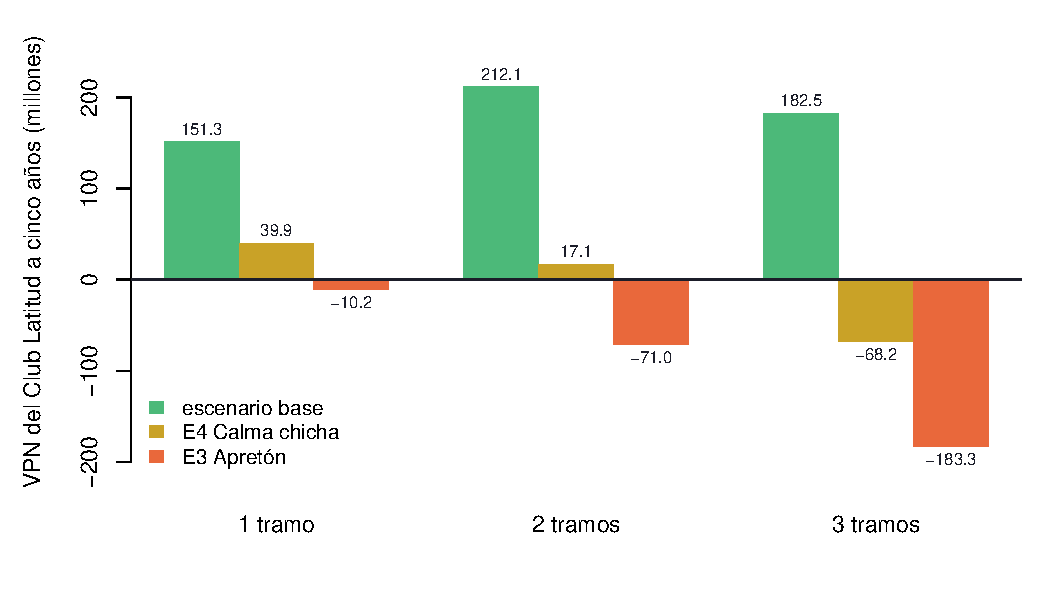
\includegraphics[width=\textwidth]{figures/tramos_club.pdf}
\end{column}
\begin{column}{0.5\textwidth}
\small
{\footnotesize
\begin{tabular}{@{}lr@{}}
\toprule
Alternativa & VPN base \\
\midrule
A, local 1 & 14.6 \\
A, local 2 & 243.5** \\
A, local 3 & $-488.3$ \\
B, 1 tramo & 151.3 \\
B, 2 tramos & \textbf{212.1} \\
B, 3 tramos & 182.5 \\
C, el piloto & $-107.0$ \\
D, esperar & 0 \\
\bottomrule
\end{tabular}}
\medskip

El tercer tramo resta 29.6: los últimos quinientos suscriptores cuestan 300.000 pesos cada uno. El local 2 lleva asterisco doble (arriendo fuera del rango, hoja de diez puntos de venta). C vale $-107$ hoy: 120 por una opción que vale 13. Y eso es un solo futuro.
\end{column}
\end{columns}
\end{frame}

\begin{frame}{La tabla de robustez de referencia: quién gana dónde}
\centering
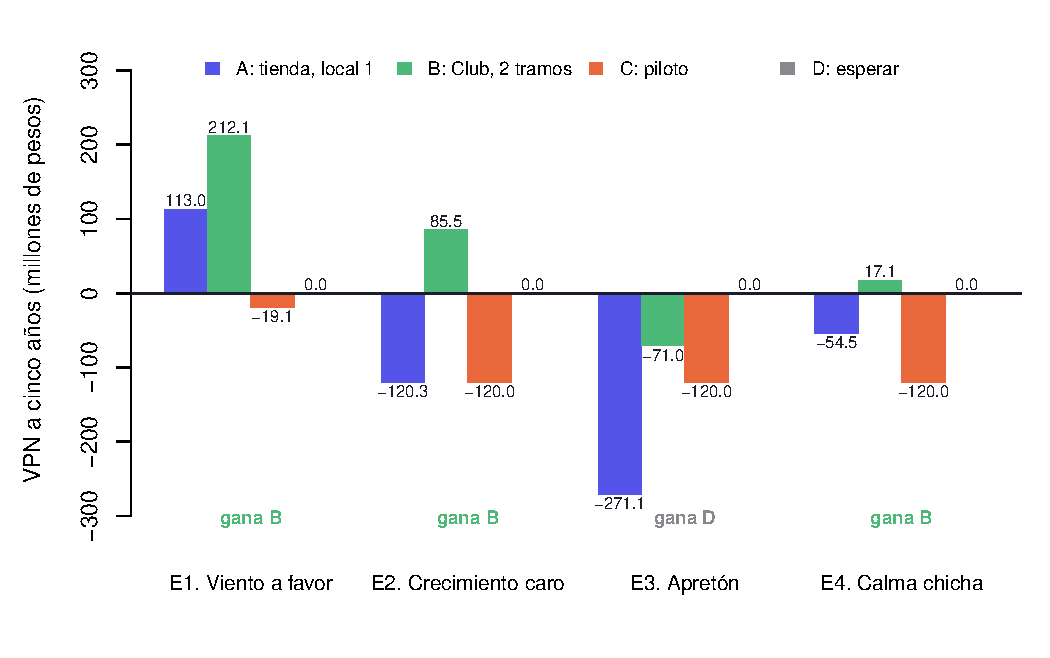
\includegraphics[width=0.84\textwidth]{figures/robustez_referencia.pdf}
\par\vspace{-2pt}
\raggedright
\footnotesize A con el local 1, B con dos tramos. B gana en tres de cuatro; D gana en Apretón, donde nada rinde; A pierde en tres y hasta 271.1; C no gana en ninguno. Su valor está en otra parte.
\end{frame}

\begin{frame}{El arrepentimiento: lo que cada alternativa deja de ganar}
\begin{columns}[T]
\begin{column}{0.58\textwidth}
{\scriptsize\setlength{\tabcolsep}{3.5pt}
\begin{tabular}{@{}lrrrrr@{}}
\toprule
 & E1 & E2 & E3 & E4 & Máximo \\
\midrule
A, local 1 & 99.1 & 205.7 & 271.1 & 71.6 & 271.1 \\
B, 2 tramos & 0.0 & 0.0 & 71.0 & 0.0 & \textbf{71.0} \\
C, el piloto & 231.2 & 205.5 & 120.0 & 137.1 & 231.2 \\
D, esperar & 212.1 & 85.5 & 0.0 & 17.1 & 212.1 \\
\bottomrule
\end{tabular}}
\medskip

\footnotesize Arrepentimiento = el mejor VPN del escenario menos el de la alternativa. La robusta minimiza el máximo: B, que en el peor de sus futuros deja de ganar 71.0.
\end{column}
\begin{column}{0.42\textwidth}
\importa{¿Por qué no promediar? El promedio de A en los cuatro es cerca de $-83$: un número que no ocurre en ningún futuro, que supone probabilidades iguales que nadie declaró, y que borra lo que la junta necesita saber: que A vale 113 o pierde 271 según dos variables que no controla.}
\end{column}
\end{columns}
\end{frame}

\begin{frame}{Esperar y pilotear: el análisis de banda}
\centering
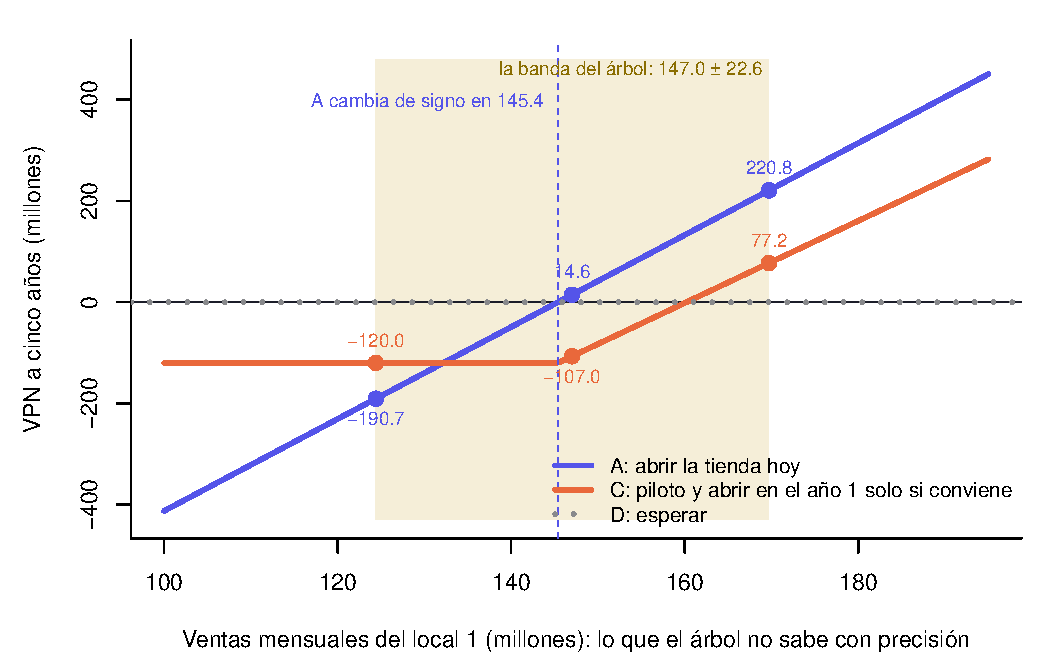
\includegraphics[width=0.82\textwidth]{figures/banda_abcd.pdf}
\par\vspace{-2pt}
\raggedright
\footnotesize En la banda baja (124.4) A pierde 190.7 y C 120.0; en la alta (169.7) A vale 220.8 y C 77.2. El piloto limita el peor caso a cambio de ceder parte del mejor: \textbf{compra el signo de A}, que es lo que el árbol no sabe. D vale 0 en los tres.
\end{frame}

\begin{frame}{El giro: el futuro cambió}
\begin{columns}[T]
\begin{column}{0.58\textwidth}
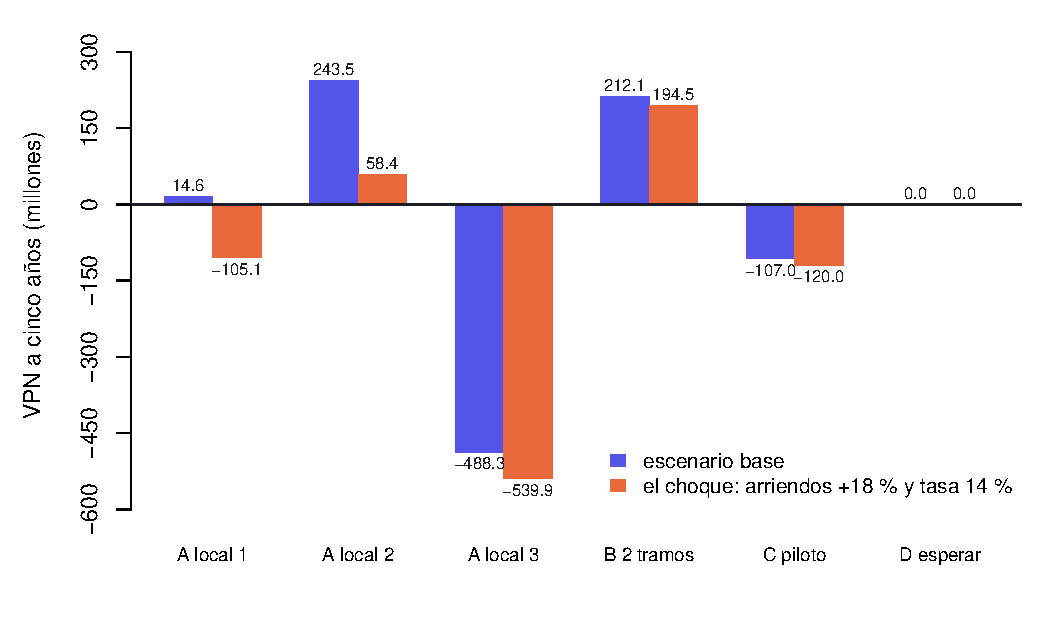
\includegraphics[width=\textwidth]{figures/choque.pdf}
\end{column}
\begin{column}{0.42\textwidth}
\parada{el giro}{Arriendos $+18$\,\% (el impulsor de la semana 2) y tasa 14\,\% (Banrep volvió a subir). Tres minutos por equipo: ¿qué recomendaciones sobreviven?}
\medskip
\footnotesize A local 1: de 14.6 a $-105.1$ (el arriendo solo, $-75.3$; la tasa sola, $-19.4$). B con dos tramos: de 212.1 a 194.5. C: $-120.0$. D: 0. \textbf{Sobreviven B y D.} Una recomendación que no sobrevive un choque de dos supuestos era una apuesta a que los supuestos no cambiaran.
\end{column}
\end{columns}
\end{frame}

\begin{frame}{Los disparadores, con dueño}
\footnotesize
Qué se vería primero si un escenario está llegando, y qué se hace entonces.

{\scriptsize\setlength{\tabcolsep}{3pt}
\begin{tabular}{@{}L{2.9cm}L{1.9cm}L{1.4cm}L{1.6cm}L{2.6cm}@{}}
\toprule
Indicador & Umbral & Frecuencia & Dueño & Acción \\
\midrule
Arriendo pedido por m$^2$, norte de Barranquilla (portal) & $+10$\,\% interanual & mensual & gerencia de expansión & congelar la firma; recalcular A o pasar a C \\
Ventas reales del comercio minorista (DANE) & variación anual negativa tres meses & mensual & gerencia financiera & activar ``se estanca'': recalcular con $-3$\,\% \\
Costo de adquisición por suscriptor (Club) & $>$ 200.000 pesos en el tramo 1 & quincenal & gerencia comercial & parar antes del segundo tramo \\
Tasa de política (Banrep) & 11\,\% o más & cada junta del Banco & gerencia financiera & recalcular con 14\,\%: A deja de valer \\
Inflación anual de alimentos (DANE, IPC) & más de 8\,\% & mensual & operaciones & márgenes 27\,\% y 20\,\%; renegociar con proveedores \\
\bottomrule
\end{tabular}}
\smallskip

\importa{Sin acción es una alarma que nadie atiende; sin dueño, una alarma que nadie oye.}
\end{frame}

\begin{frame}{Opcional: ponerle ruido a los supuestos}
\begin{columns}[T]
\begin{column}{0.55\textwidth}
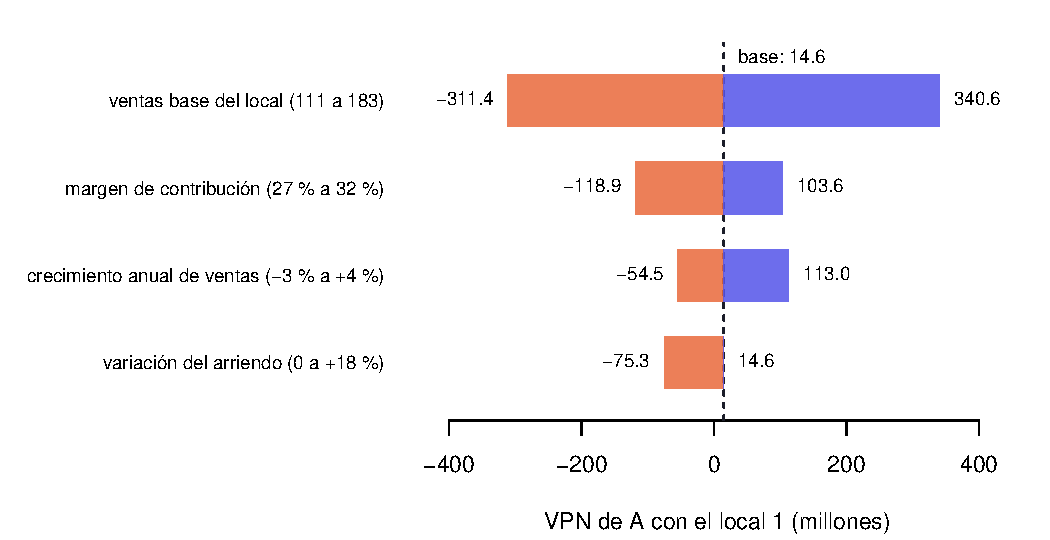
\includegraphics[width=\textwidth]{figures/tornado_A.pdf}
\end{column}
\begin{column}{0.45\textwidth}
\footnotesize
Mil corridas sobre el base: ventas base $\sim$ Normal(147, 28), crecimiento entre $-3$\,\% y $+4$\,\%, margen entre 27\,\% y 32\,\%, arriendo entre 0 y $+18$\,\%, retención entre 62\,\% y 75\,\%, suscriptores $\times$ 0.75 a 1.10.

\smallskip
A pierde en el 59\,\% de las corridas (P10 $-364.7$, P50 $-50.1$, P90 308.1); B con dos tramos, en el 0.1\,\% (62.5, 156.7, 251.8).

\smallskip
\textbf{El tornado:} las ventas base recorren 651.9; el margen 222.6; el crecimiento 167.5; el arriendo 89.9. Manda lo único que un piloto puede medir.

\smallskip
No son probabilidades de los escenarios: es ruido sobre los parámetros dentro de un futuro, y las distribuciones también van al libro de supuestos.
\end{column}
\end{columns}
\end{frame}

\begin{frame}{Lo que importa}
\importa{%
\begin{enumerate}\itemsep5pt
  \item \textbf{Un escenario es una tabla de supuestos.} Nombre, cuatro líneas y cada parámetro con valor, fuente y calidad. Sin probabilidad, sin promedio, sin ``el más probable''.
  \item \textbf{La vara es el VPN con una sola plantilla.} Cinco años, 12\,\%, 30\,\% de impuesto; un millón mensual de ventas vale 9 millones. A con el local 1 vale 14.6: cero.
  \item \textbf{La tabla de robustez decide.} Quién gana dónde, qué pierde menos, el arrepentimiento máximo. B es robusta con 71.0; D gana en Apretón; A se arrepiente hasta 271.1.
  \item \textbf{Pilotear compra el signo; esperar no es gratis; el disparador tiene dueño.} La banda cruza el cero: C limita el peor caso a $-120$. Y lo que no aguanta el choque no era una recomendación.
\end{enumerate}}
\end{frame}

\seccion{El task y el cierre}
%% ====================================================== 3. PUENTE (65–70)
\begin{frame}{Task 7: escenarios, robustez y disparadores}
\begin{columns}[T]
\begin{column}{0.55\textwidth}
\small
\textbf{Qué se entrega} (una página más el anexo, en equipo, antes de la sesión 8; con la práctica 7, sin código):
\begin{itemize}\itemsep3pt
  \item tres o cuatro escenarios desde sus dos incertidumbres del task 2: nombre, cuatro líneas, tabla de supuestos con fuente y calidad (2.0);
  \item la tabla de robustez de A, B, C y D con su local y sus tramos: el base contra el sobre, ganador por escenario, arrepentimiento máximo (1.5);
  \item la recomendación en seis líneas y tres disparadores (1.0);
  \item el acta y la declaración (0.5).
\end{itemize}
\end{column}
\begin{column}{0.45\textwidth}
\small
\begin{exampleblock}{En el cierre de la sesión 8}
La tabla de robustez y los disparadores en pantalla. ¿Qué sobrevive el choque? ¿Qué disparadores se repiten?
\end{exampleblock}
\begin{alertblock}{Lo que no cuenta}
Un escenario con probabilidad. Un parámetro sin fuente ni ``supuesto del equipo''. Un VPN base que no coincida con el sobre sin explicar. Más de cuatro líneas por escenario. ``Todo sigue igual'' como único escenario.
\end{alertblock}
\end{column}
\end{columns}
\end{frame}

\begin{frame}{El encargo: la entrevista al experto}
\begin{columns}[T]
\begin{column}{0.5\textwidth}
\small
\textbf{A quién.} Alguien que conoce el negocio de primera mano: un gerente de expansión o de operaciones de una cadena de comercio, un corredor de locales comerciales en Barranquilla o un gerente de un programa de suscripción o de comercio electrónico. Veinte minutos.

\medskip
\textbf{Cuándo.} Entre esta semana y la sesión 8. Se registra en el task 8.

\medskip
\textbf{Qué se pregunta.} Tres preguntas fijas: ¿qué de estos escenarios le parece inverosímil?, ¿qué supuesto cambiaría?, ¿qué haría usted con los \peso1.000 millones? Y tres sobre los parámetros de \textbf{calidad baja} de su tabla.
\end{column}
\begin{column}{0.5\textwidth}
\begin{block}{Cómo se registra}
Tres reacciones textuales (una línea cada una), qué fila de la tabla de supuestos cambió por ellas, y qué no cambió y por qué. El experto valida los supuestos; no decide por el equipo.
\end{block}
\small En el cierre de la sesión 8, cada equipo dice con quién fue y cuándo.
\end{column}
\end{columns}
\end{frame}

%% ====================================================== 4. CIERRE (70–90)
\begin{frame}{Cierre: ¿cuánto vende? (task 6)}
\begin{enumerate}\itemsep6pt
  \item \textbf{Encuesta} (2 minutos): ¿le ganamos a la regla del sector? A mano alzada: quién tiene un árbol con MAE menor que 22.4 en validación, por más que el margen.
  \item \textbf{Dos equipos al azar, dos minutos cada uno} (6 minutos): su tabla del líder en pesos y dónde falla su árbol. Referencia: profundidad 3, MAE 22.6; la regla 8 $\times$ arriendo, 22.4; empate técnico.
  \item \textbf{Las bandas de los tres locales} (8 minutos): se comparan entre equipos. Referencia: local 1 147.0 [124.4, 169.7], local 2 207.2 [184.5, 229.8] con asterisco doble, local 3 63.3 [40.6, 85.9]. ¿Qué equipo tiene una banda que cruza las ventas de equilibrio (145.4)? Esa es la pregunta del piloto.
  \item \textbf{La posición actualizada} (2 minutos): ¿quién cambió de alternativa desde la semana 1 y por qué cifra?
  \item \textbf{Dudas} (2 minutos): la práctica 7, el sobre y la entrega del task 7.
\end{enumerate}
\end{frame}

\begin{frame}{Referencias}
\small
\begin{itemize}\itemsep4pt
  \item Wack, P. (1985). Scenarios: uncharted waters ahead. \emph{Harvard Business Review}, 63(5), 72--89.
  \item Wack, P. (1985). Scenarios: shooting the rapids. \emph{Harvard Business Review}, 63(6), 139--150.
  \item Schoemaker, P. J. H. (1995). Scenario planning: a tool for strategic thinking. \emph{Sloan Management Review}, 36(2), 25--40.
  \item Sosa Escudero, W. (2014). \emph{Qué es (y qué no es) la estadística}. Siglo XXI. El capítulo sobre predicción e incertidumbre.
\end{itemize}
\end{frame}

\end{document}
